\documentclass{article}
\usepackage[utf8]{inputenc}
\usepackage[english,russian]{babel}
\usepackage{graphics}
\usepackage{amsmath}
\usepackage{graphicx}
\graphicspath{{./pic/}}

\begin{document}
	N7.\\
	Постройте график функции:\\
	\begin{equation*}
		y(x) = 
		\begin{cases}
			x^2-6x+13, x \geq 2\\
			2,5x, x < 2\\
		\end{cases}
	\end{equation*}\\
	и определите, при каких значениях m прямая y = m имеет с графиком ровно две общие точки.\\
	\begin{figure}[h!]
		\begin{center}
			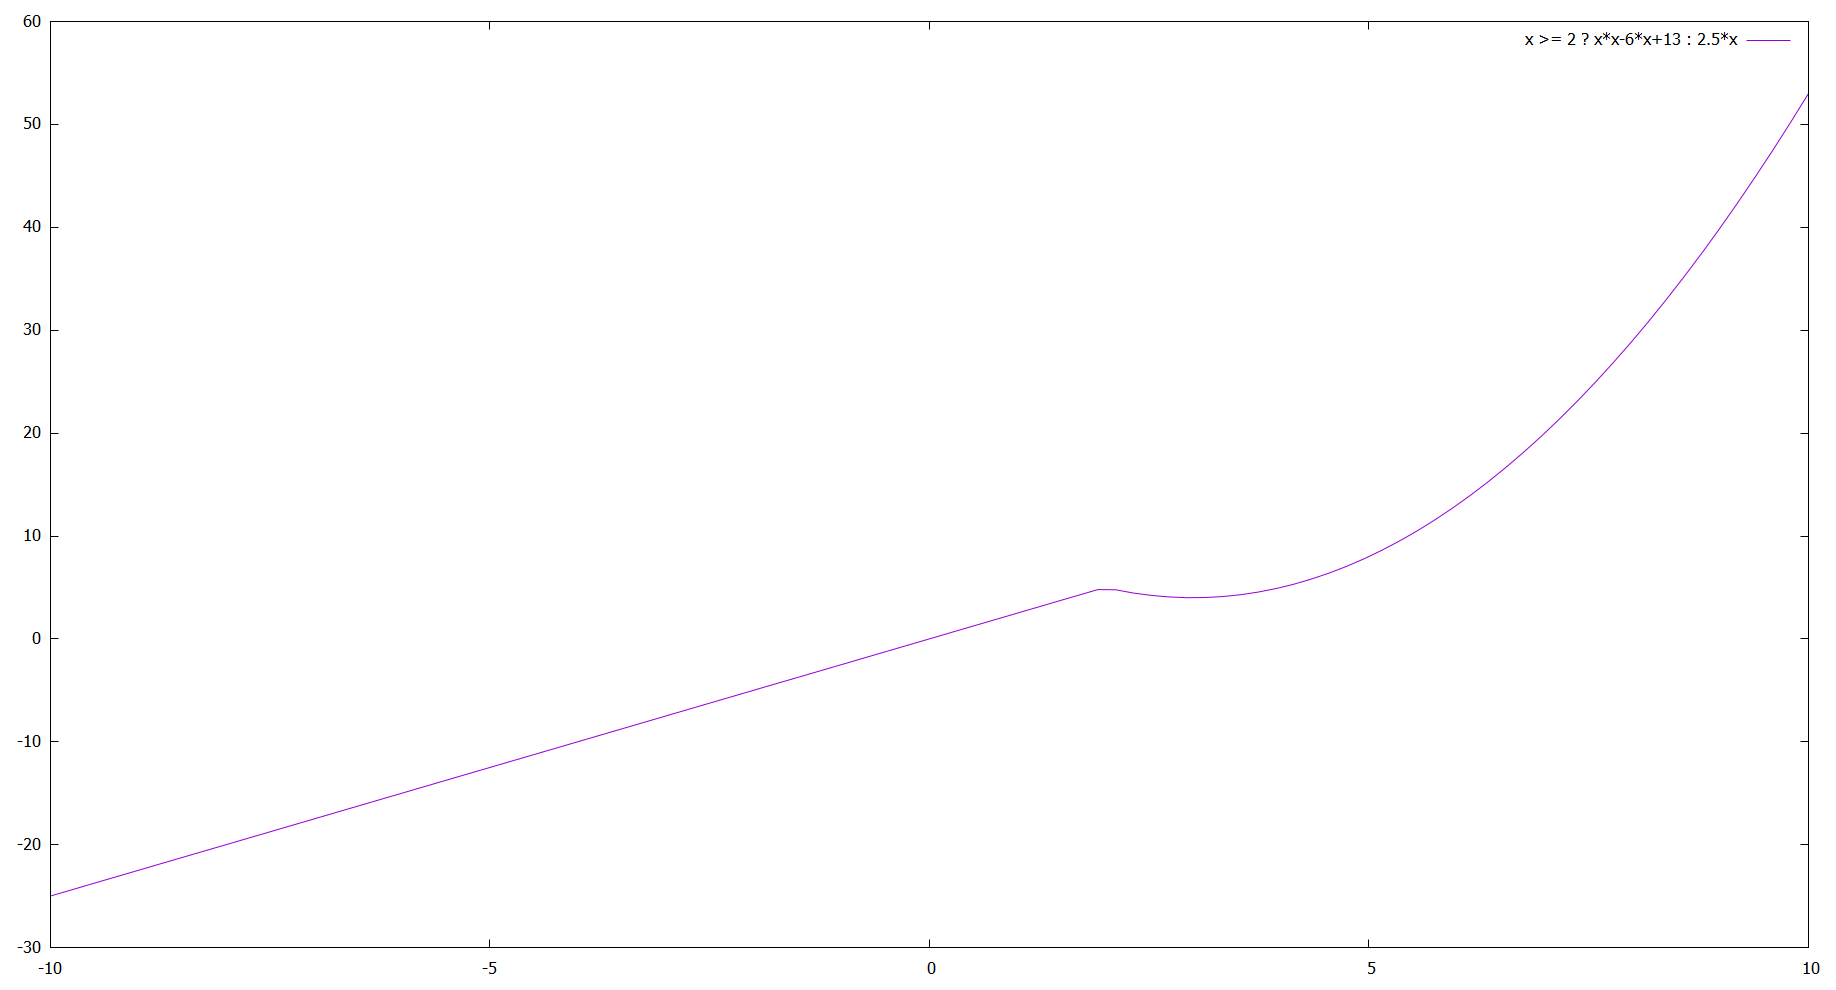
\includegraphics[scale=0.2]{N7 graphic 1}
		\end{center}
	\end{figure}\\
	Сначала найдём наименьшее значение функции $x^2-6x+13, x \geq 2$\\
	$x_{0} = -(-6)/2=3, y_{0} = 3^2-6*3+13=4$\\
	\\
	Теперь найдём максимальное значение функции $2,5x, x < 2$\\
	Так как функция монотонно возрастает, то $y=max$ при $x=max$. Значит $y=5$ при $x=2$\\
	\\
	Построим две прямые $y=4$ и $y=5$:\\
	\begin{figure}[h!]
		\begin{center}
			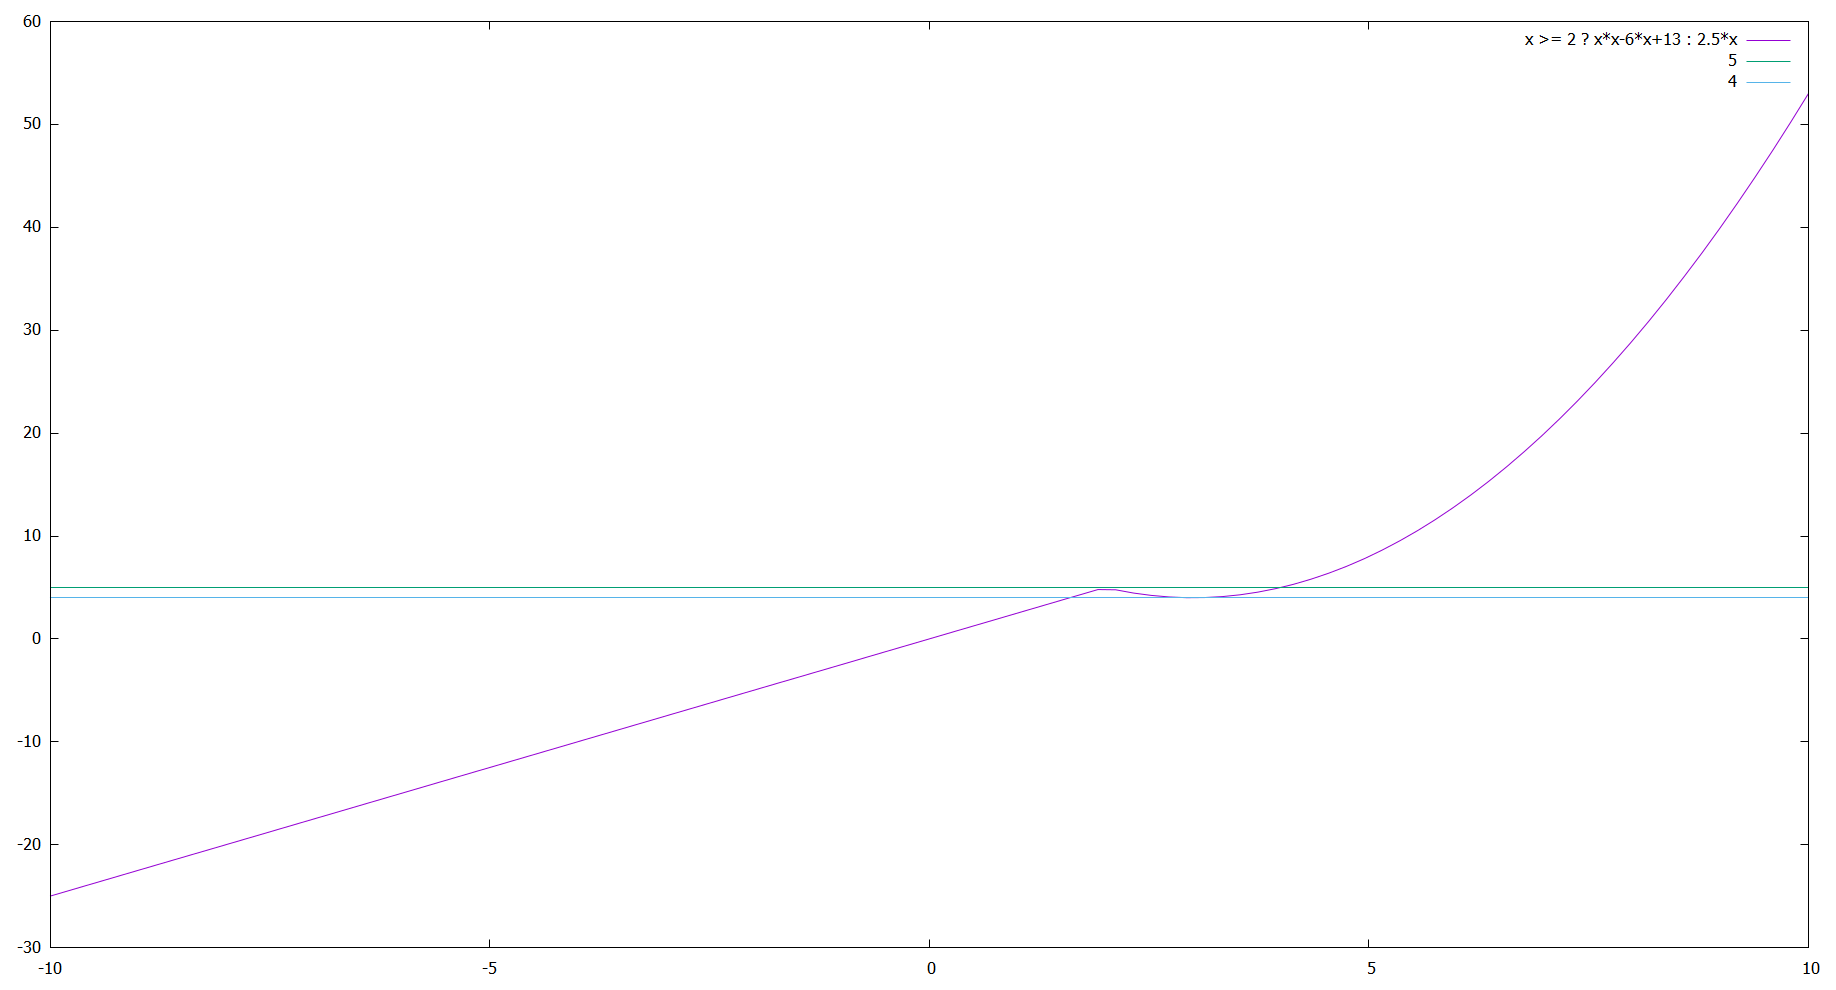
\includegraphics[scale=0.2]{N7 graphic 2}
		\end{center}
	\end{figure}\\
	\\
	\\
	\\
	\\
	\\
	\\
	\\
	\\
	\\
	Как мы видим если $y < 5$ и $y>4$, то прямая $y=m$ имеет 3 общие точки с графиком, а если $y > 5$ или $y < 4$, то прямая $y = m$ имеет 1 общую точку с графиком.\\
	\\
	Ответ: $y = 5$ или $y = 4$
\end{document}
